\documentclass{article}%You can define the type of paper here.
%%Useful packages that I commonly use.
\usepackage[numbers]{natbib}%Bibliography package (help at http://merkel.zoneo.net/Latex/natbib.php).
\usepackage{url}%Package to highlight url.
\usepackage{times}%Sets font to be times.
\usepackage{alltt}%Allows the use of verbatim (good for printing out code).
\usepackage{graphicx}%Used to import images.
\usepackage{amsmath, amssymb, amscd}%Contains the AMS expanded math symbols library.
%%For those who want smaller margins, you can use this:
\usepackage[top=1in, bottom=1in, left=1in, right=1in]{geometry}

\begin{document}

    %%Title
    \title{Simulation and Modeling\\Project I: Bullet Drag}
    \author{Clinton McKay}
    \maketitle

    %%Makes the paper use two collums
    \twocolumn

    %%Introduction-------------------------------------------------------------------------------------
    \section{Introduction}
    Ammunition manufacturers when selling their cartridges, will provide the relevant data to their customers. The data provided contains; trajectories, velocities, bullet mass, and the ballistic coefficient. This data allows hunters to assess the trajectories of the ammunition they have bought. Using this data, the project will focus on simulating various bullet trajectories given different models. The collected data will then serve as a method to decide which model is the best candidate for various bullets. 

    %%Method------------------------------------------------------------------------------------------
    \section{Method}
    Modeling the system required two main components. The first component was modeling the forces that would be acting on the bullet. The primary force formula was:

    \begin{align*}
        \mathbf{F_d} &= -\frac{A(v)}{b_c} v^{M(v)-1} \mathbf{v}\\
    \end{align*}
    
    $F_d$ models the drag on the bullet as it travels through the air at high velocities. This model is designed to be used in conjunction with a referenced round. The referenced datasets are called {\em G} models. Given the scope of this project, {\em G1}, {\em G2}, {\em G5}, {\em G7}, and {\em G8} served as the test candidates. $A(v)$ and $M(v)$ are lookup values from the active {\em G} model. $b_c$ is the drag coefficient of the bullet and $v$ is the velocity of the projectile. 

    The previous equation properly models the drag, but it does not provide a complete model to all of the forces acting on the bullet. The second component forces us to compensate for gravity, resulting in a further breakdown of the function. The forces acting in the $y$ direction of the bullet now include the force of gravity. 
    
    \label{eq:drag}
    \begin{align*}
        a_x &=& - \frac{A(v)}{b_c} v^{M(v)-1}v_x\\         
        a_y &=& - g - \frac{A(v)}{b_c} v^{M(v)-1}v_y\\ 
    \end{align*}

    Besides focusing on the implementation of the {\em G} models. The project required the implementation a custom drag force formula $F_d$. 
    
    \begin{align*}
        \mathbf{F}_d= -{1 \over 2} \rho v^2 A C_d(v) \mathbf{\hat v}
    \end{align*}

    The new formula is structured such that it compensates for the density of the fluid the projectile is traveling through ($\rho$). $A$ is the cross-sectional area of the projectile. $v$ is the velocity of the projectile and $C_d$ is the drag coefficient. Since $C_d$ is dependent on the velocity, then it was necessary to produce a function that models $C_d$ based on the velocity that is passed in. The resulting function was. 
   
    \label{eq:customdrag}
    \begin{align*}
        C_d(v) = \begin{cases}
            f(x), & x\leq 1.2 \\ 
            f(1.2) - e^{-1.2} + e^{-x} * a, & x>1.2 \qquad \text{$a$ is a constant}
        \end{cases}
    \end{align*}

    Where $f(x)$ is defined as.
    
    \begin{align*}
        f\left( x \right)\; =\frac{1}{20\left( 1.534-\; x \right)^{2}} 
    \end{align*}

    %%Verification------------------------------------------------------------------------------------
    \section{Verification of Program}
    To implement the system Python the its library NumPy were used. To easily store and retrieve bullets. They have been stored in a YAML\cite{1} file for easy access. Here is a breakdown of the scripts. 
    \begin{description}
        \item[main.py] main execution script. Loads up the modules and runs the simulation. 
        \item[BallisticModel.py] Contains all of the {\em G} models and the custom model. 
        \item[BulletData.yaml] Any additional bullets go here. 
        \item[Projectile.py] Contains the Projectile class and all of the necessary functions to simulate a bullet trajectory and zero in on a target. 
    \end{description}

    The two main components of the program are located in {\bf Projectile.py} and {\bf BallisticModel.py}. 
    {\bf Projectile.py} contains the {\em zero\_in} function and the {\em Projectile.move} method. 

    The {\em zero\_in} function takes in a Projectile object, a starting angle $\theta$ in degrees, a distance to zero onto, a tolerance to stop at, and a ratio r. With these arguments, {\em zero\_in} will continue iterating until firing at angle $\theta$ "hits" the target at the zero distance. The value of theta is determined by the following formula. 

    \begin{align*}
       \theta_k = \begin{cases}
            \theta_{k - 1} - r^k\theta_{k - 1}, y \geq 0\\
            \theta_{k - 1} + r^k\theta_{k - 1}, y < 0\\
        \end{cases}
    \end{align*}

    $y$ is the distance from zero at the zero-in distance. $k$ is the iteration count. 

    {\em Projectile.move} contains the ODE system that models the motion of the projectile as described in equations \ref{eq:drag}. 

    The final component is within the {\bf BallisticModel.py} module. The various {\em G} and custom models are located in this module. The {\em Custom\_Module} class contains an implementation of the custom drag formula. 

    %%Data--------------------------------------------------------------------------------------------
    \section{Data}
    The bullets used to compare the different models was the .308 Remington Winchester and the .338 Lapua Magnum. 

    \begin{description}
        \item[.308 Remmignton Winchester]\mbox{ }
            \begin{description}
                \item[grains] 150 grains
                \item[ballistic coefficient] 0.314
                \item[Muzzle Velocity] 2820 $^{ft}/_s$
                \item[Long-range trajectory] \mbox{ }
                \begin{table}[h!]
                \center
                    \begin{tabular}{c|c}
                        Distance (yd) & Height (in) \\ \hline
                        100 & 2 \\
                        150 & 1.7 \\
                        200 & 0 \\
                        250 & -3.4 \\
                        300 & -8.8 \\
                        400 & -26.2 \\
                        500 & -54.8 \\
                    \end{tabular}
                \end{table}
                \item[Velocity trajectory] \mbox{ }
                \begin{table}[h!]
                \center
                    \begin{tabular}{c|c}
                        Distance (yd) & Velocity ($^{ft}/_s$) \\ \hline
                        100 & 2533 \\
                        200 & 2263 \\
                        300 & 2009 \\
                        400 & 1774 \\
                        500 & 1560 \\
                    \end{tabular}
                \end{table}
                \item[Diameter] 7.8 mm
            \end{description}
        \item[.338 Lapua Magnum]\mbox{ }
            \begin{description}
                \item[grains] 300 grains
                \item[ballistic coefficient] 0.242
                \item[Muzzle Velocity] 2723.1 $^{ft}/_s$
                \item[Long-range trajectory]\mbox{ } 
                \begin{table}[h!]
                \center
                    \begin{tabular}{c|c}
                        Distance (yd) & Height (in) \\ \hline
                        109.361 & 0 \\
                        281.723 & -4.606 \\
                        328.084 & -15.984 \\
                        656.168 & -99.370 \\
                        874.891 & -205.945\\
                        1093.61 & -365.709 \\
                    \end{tabular}
                \end{table}
                \item[Velocity trajectory]\mbox { }
                \begin{table}[h!]
                \center
                    \begin{tabular}{c|c}
                        Distance (yd) & Velocity ($^{ft}/_s$) \\ \hline
                        109.361 & 2588.58 \\
                        281.723 & 2460.63 \\
                        328.084 & 2335.96 \\
                        656.168 & 1984.91 \\
                        874.891 & 1768.37 \\
                        1093.61 & 1568.24 \\
                    \end{tabular}
                \end{table}
                \item[Diameter] 7.8 mm
            \end{description}
    \end{description}
    
    %%Analysis---------------------------------------------------------------------------
    \section{Analysis}
    The resulting trajectories were produced after running the simulation. Figure \ref{fig:308x} and \ref{fig:388x} compare the affects of different drag models on the bullet. 

    \begin{figure}[!h]  
        \centering
        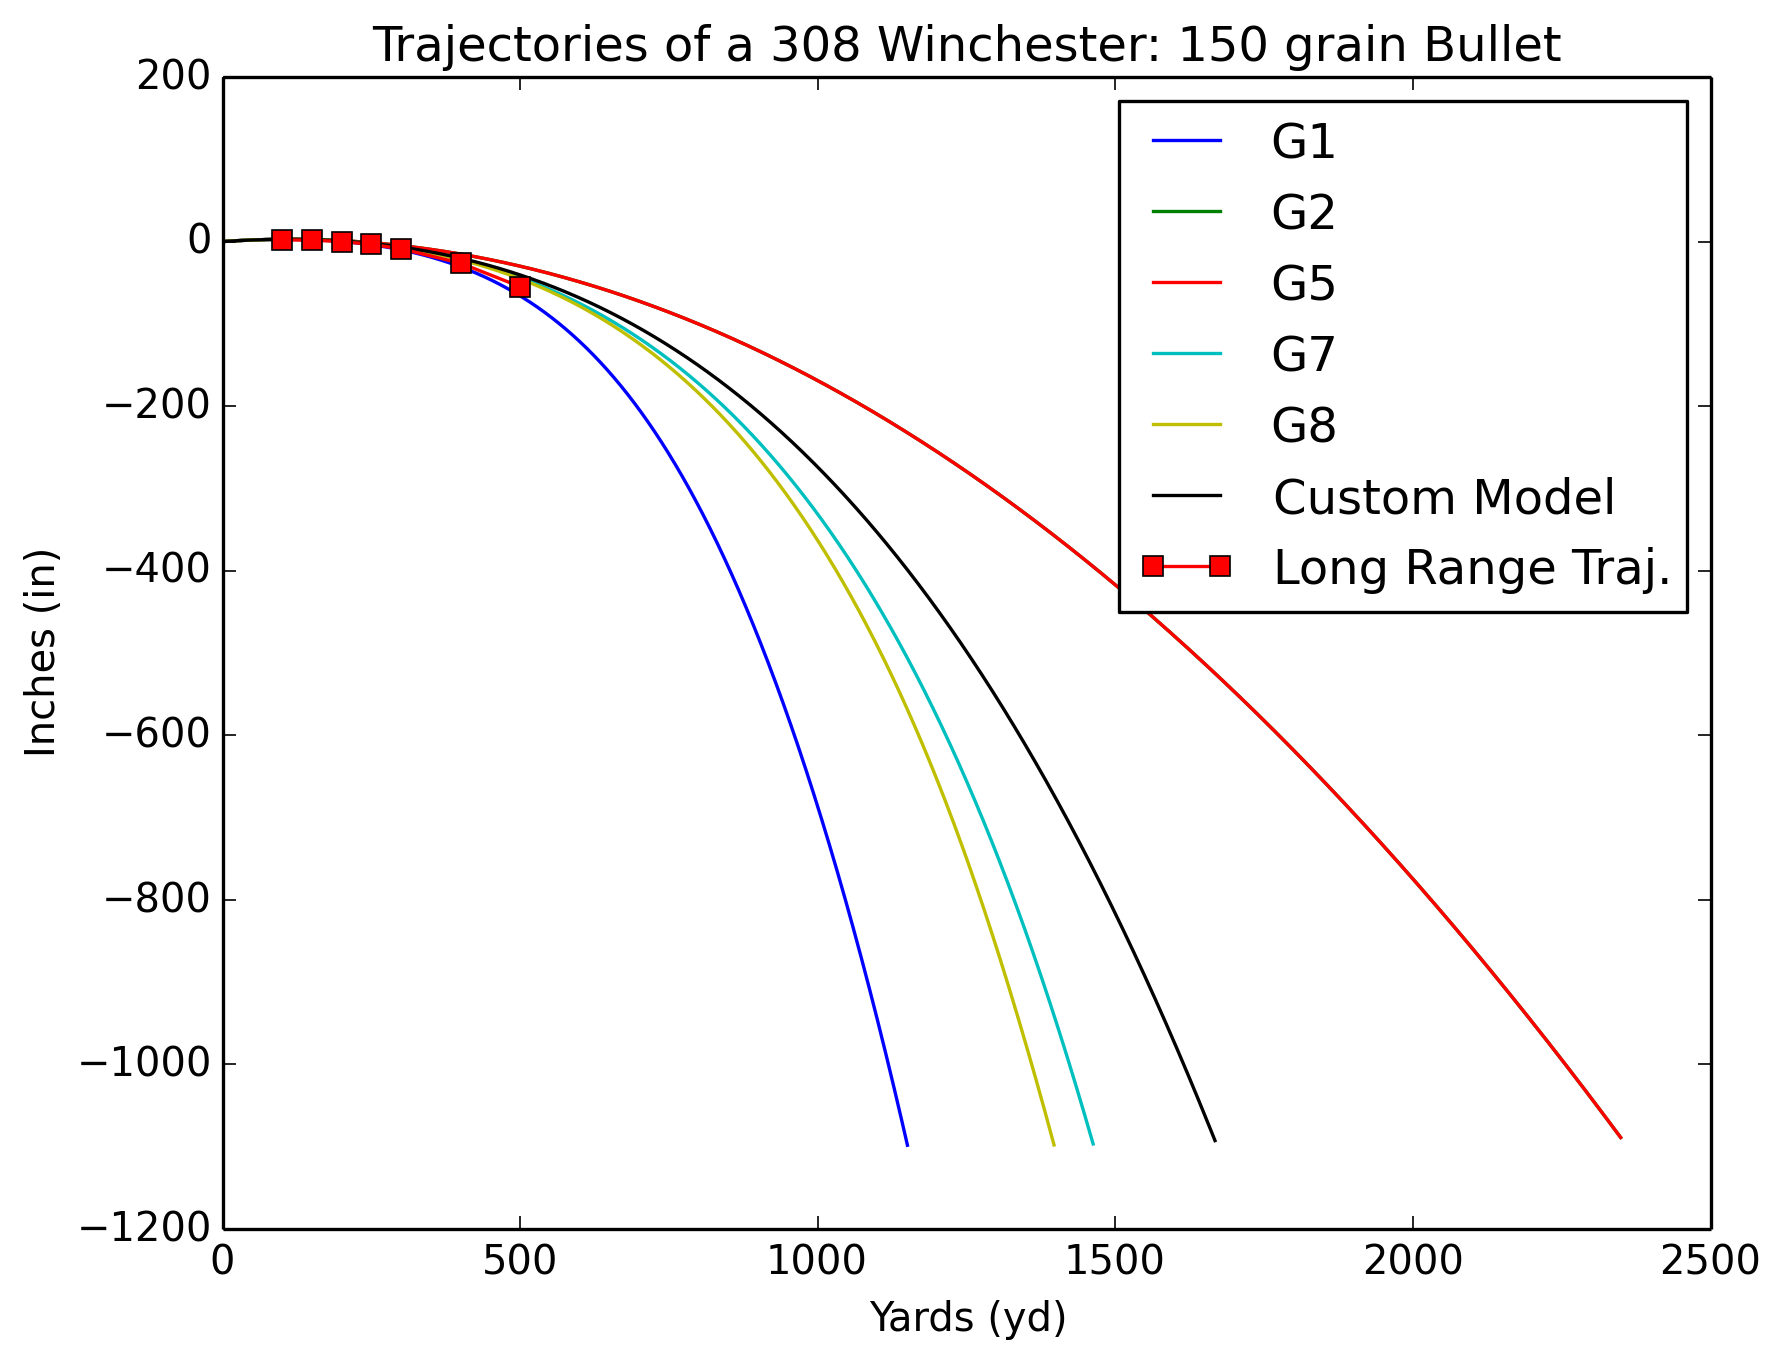
\includegraphics[width=0.48\textwidth]{../img/308-Winchester_dist_comp.png}
        \label{fig:308x}         
        \caption{Bullet trajectories of the .308 Remington Winchester using different models. }
    \end{figure}
    
    \begin{figure}[!h]  
        \centering
        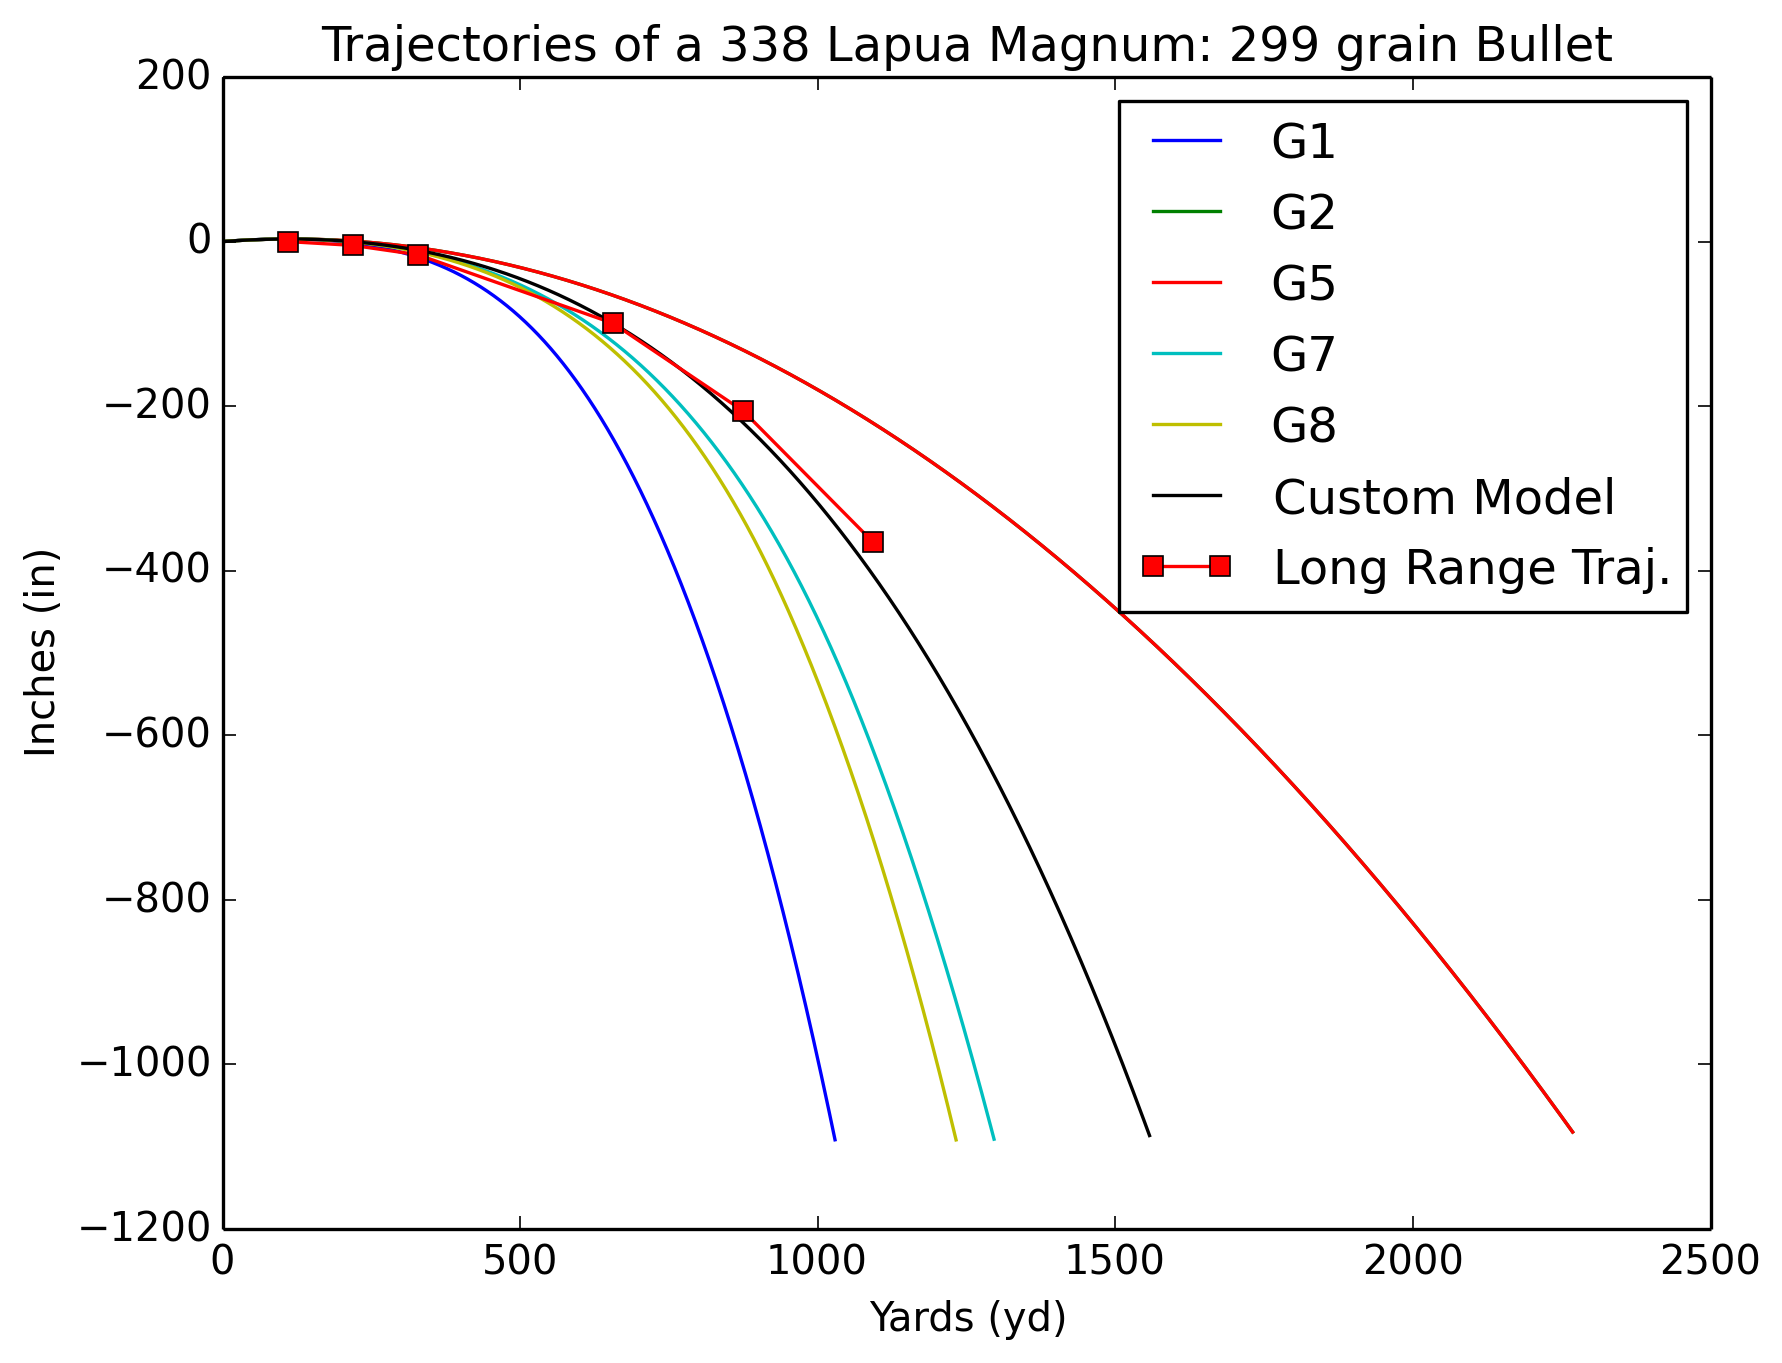
\includegraphics[width=0.48\textwidth]{../img/338-Lapua-Magnum_dist_comp.png}
        \label{fig:388x}         
        \caption{Bullet trajectories of the .338 Lapua Magnum using different models. }
    \end{figure}

    Figures \ref{fig:308v} and \ref{fig:338v} show the different velocity trajectories based on the model used. 


    \begin{figure}[!h]  
        \centering
        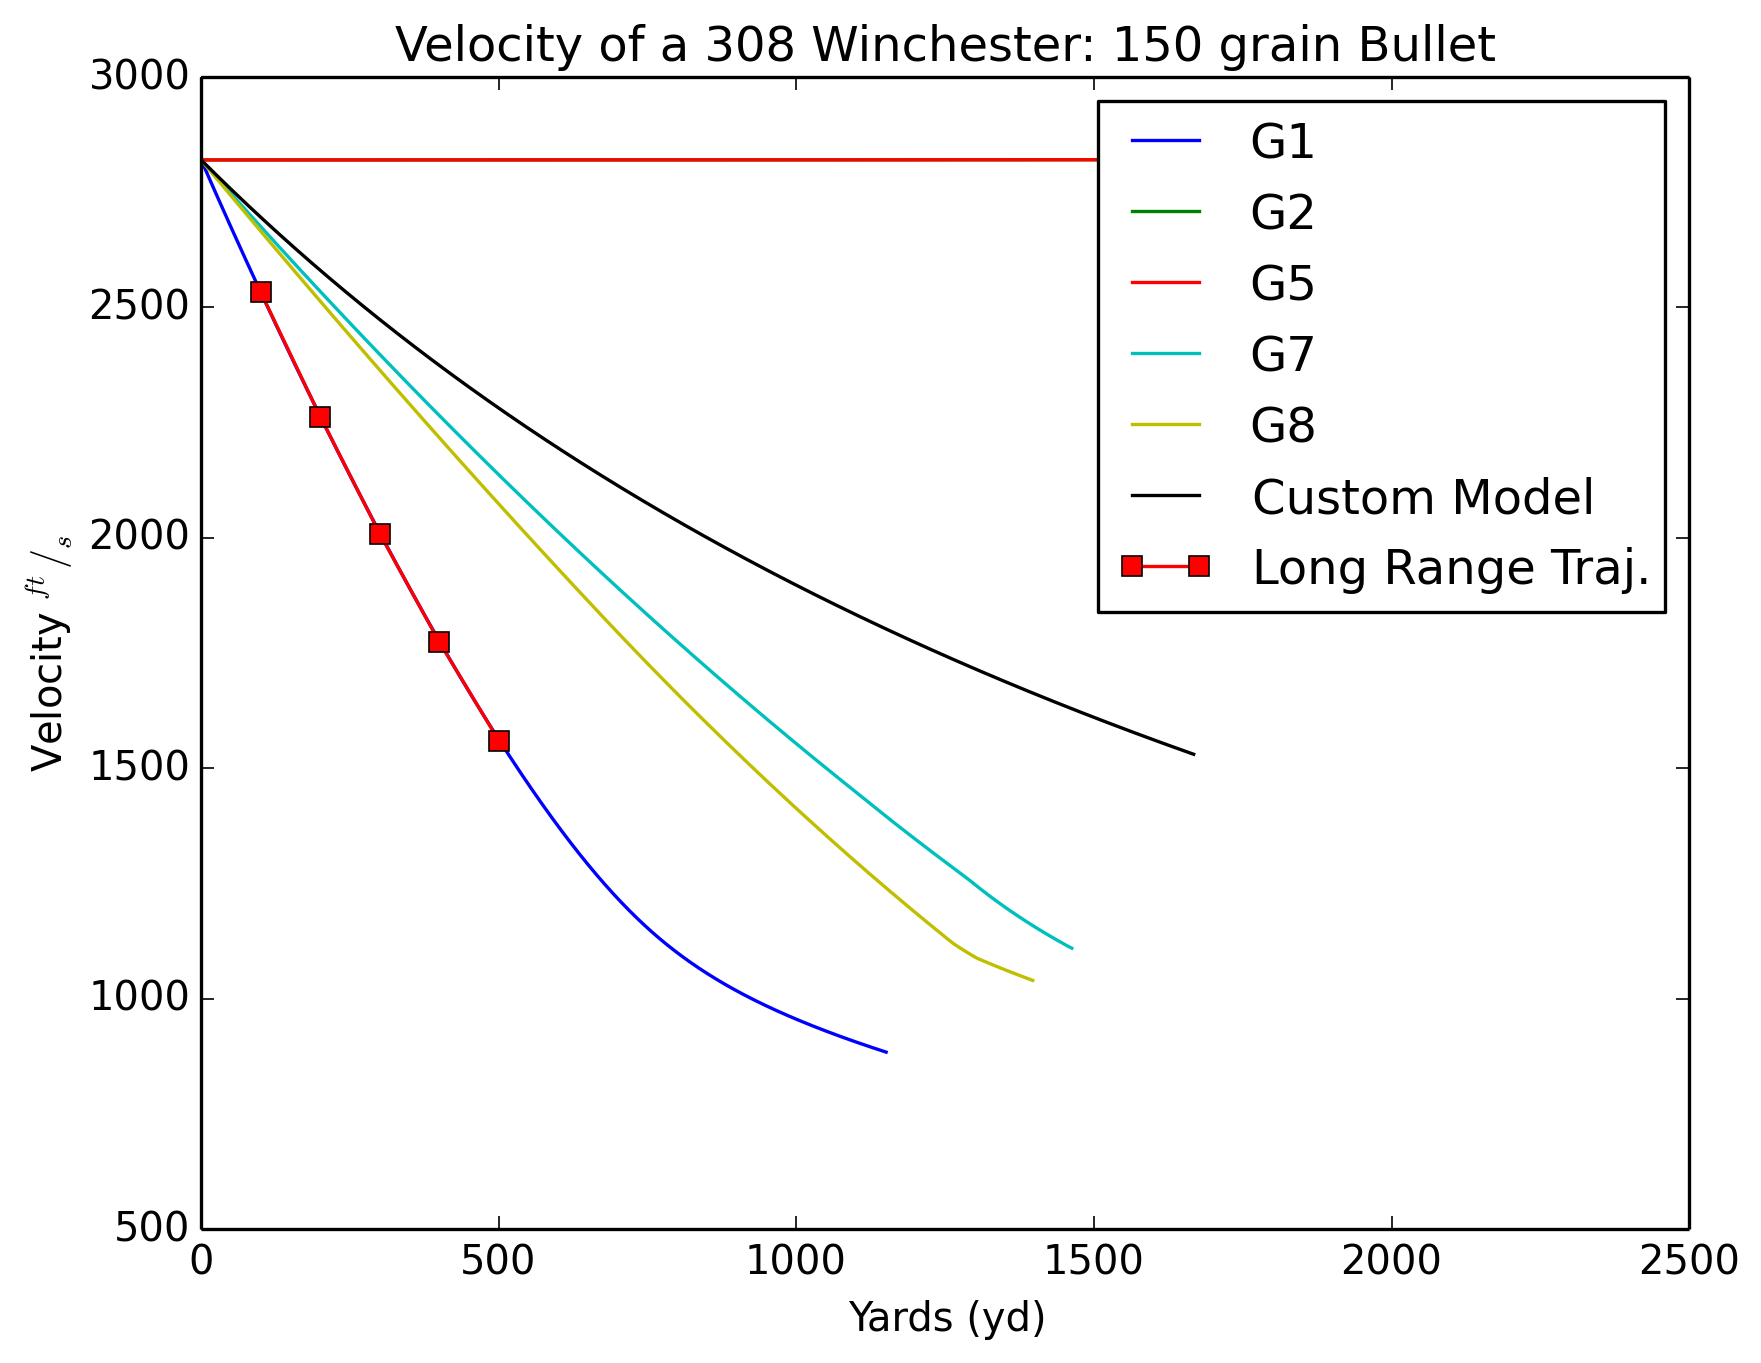
\includegraphics[width=0.48\textwidth]{../img/308-Winchester_vel_comp.png}
        \label{fig:308v}         
        \caption{Bullet trajectories of the .308 Remington Winchester using different models. }
    \end{figure}
    
    \begin{figure}[!h]  
        \centering
        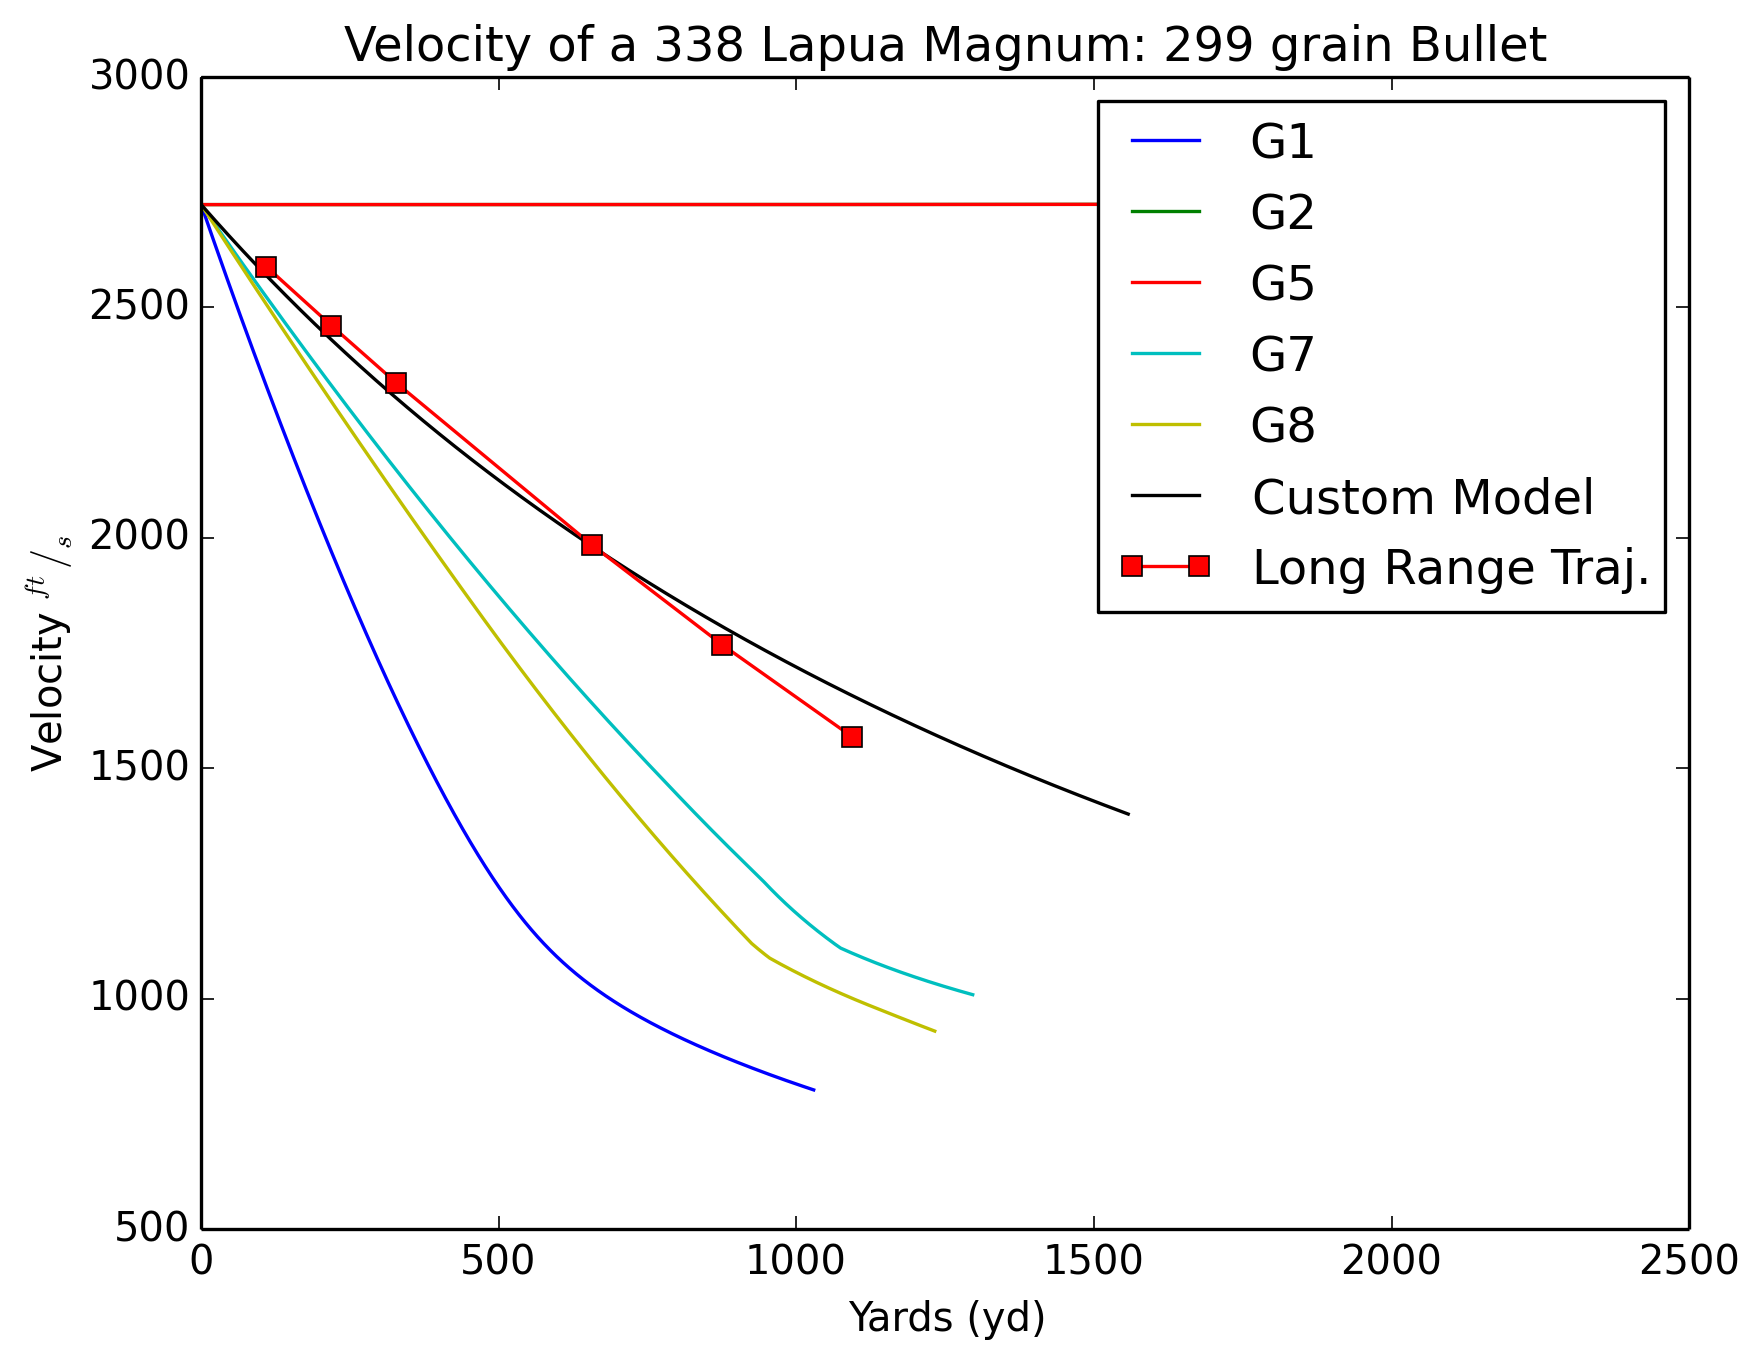
\includegraphics[width=0.48\textwidth]{../img/338-Lapua-Magnum_vel_comp.png}
        \label{fig:338v}         
        \caption{Bullet trajectories of the .338 Lapua Magnum using different models. }
    \end{figure}

    %%Interpretation---------------------------------------------------------------------
    \section{Interpretation}

    What was interesting was the custom model performed the best for the 338 rounds, but it was the second worst model when used against the Remington rounds. Perhaps this effect was due to the higher mass and the shape of the bullet. Judging by the distance that the 338 traveled it must of had a more aerodynamic design since the custom model was able to fit its velocity and hight better. 

    The best candidate model for the 308 appears to be the {\em G1} model. Judging from these results, it may be safe to assume that the bullet creates more drag since it weighs less and is not as aerodynamic. 
    
    Instead of visually inspecting the trajectories and comparing them to the manufacturer supplied trajectories. Calculating a squared sums error between the simulated and actual trajectory would of provided more insight as to which model best fits the data. 

    %%Critique---------------------------------------------------------------------------
    \section{Critique} 

    %%Bibliography-----------------------------------------------------------------------
    \begin{thebibliography}{1}
    %        \bibitem{1}Gould, H., Tobochnik, J., \& Christian, W. (2007). \textit{An Introduction to Computer Simulation Methods: Applications to Physical Systems}. San Francisco, CA: Pearson Education, Inc.
            \bibitem{2}\url{http://www.yaml.org/}
            \bibitem{3}\url{http://wiki.cs.umt.edu/classes/cs477/index.php/Bullet_Drag}
    \end{thebibliography} 

\end{document}
